\documentclass{jsarticle}
\usepackage[dvipdfmx]{graphicx}
\usepackage{listings}
\usepackage{afterpage}
\begin{document}
\title{課題4 画像のヒストグラム}
\author{13EC060 武澤 裕介}
\maketitle
\begin{abstract}
まずmatlabを用いて画像のヒストグラムを表示、考察する。また付録としてpythonで書いた画像ヒストグラムの表示をするコードを記載する。
\end{abstract}
\section{画像のヒストグラム}
まず、今回使用する原画像を図1に示す。


\begin{figure}[htbp]
 \begin{center}
  
\includegraphics[width=5cm,height=5cm]{img_02.jpg}
 \end{center}
 \caption{原画像}
\end{figure}

\begin{lstlisting}[basicstyle=\ttfamily\footnotesize, frame=single]
filename = uigetfile('*');
ORG=imread(filename); % 原画像の入力
ORG = rgb2gray(ORG); colormap(gray); colorbar;
imagesc(ORG); axis image; % 画像の表示
pause; % 一時停止
 \end{lstlisting}
を用いてまず入力画像のグレースケール画像を表示させる。

\newpage
\begin{figure}[htbp]
 \begin{center}
  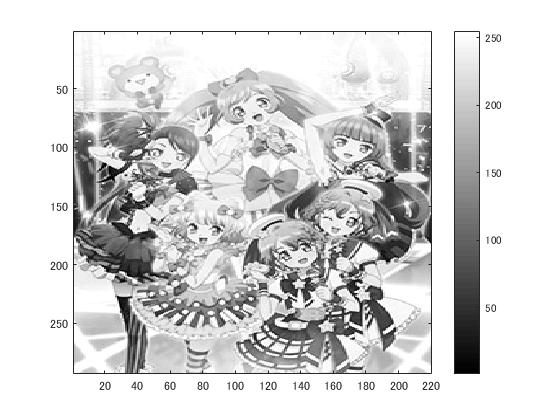
\includegraphics[width=10cm]{kadai4-0.jpg}
 \end{center}
 \caption{グレースケール画像}
\end{figure}

最後に
\begin{lstlisting}[basicstyle=\ttfamily\footnotesize, frame=single]
imhist(ORG); % ヒストグラムの表示
 \end{lstlisting}
を用いて画像の輝度ヒストグラムを表示する。

\newpage
\begin{figure}[htbp]
 \begin{center}
  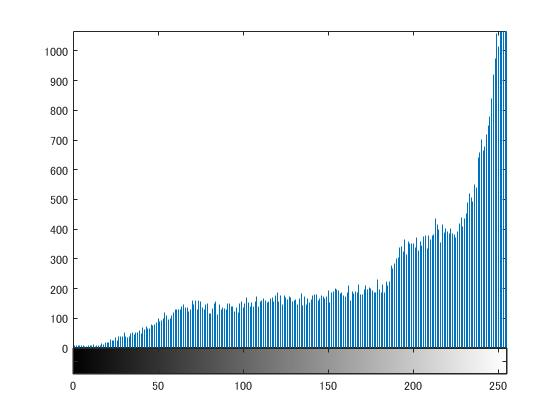
\includegraphics[width=10cm]{kadai4-1.jpg}
 \end{center}
 \caption{輝度ヒストグラム}
\end{figure}

\section{考察}
図3の画像の輝度ヒストグラムから比較的今回使用した画像には輝度値の高い画素が輝度値が低い画素よりも比較的に含まれていることが分かった。つまり一般的には画像が明るく見える。実際今回使用した画像は全体的に明るく見えていると言える。

\newpage
\section{付録-python2.x系列による画像のヒストグラム表示コード-}
\begin{lstlisting}[basicstyle=\ttfamily\footnotesize, frame=single]
#-*-coding:utf-8-*-
import cv2
import pylab as plt
import sys
import matplotlib.font_manager

argvs=sys.argv  
if (len(argvs) != 2):  
    print 'Usage: # python %s filename' % argvs[0]  
    quit()   
  
imagefilename = argvs[1]  
try:  
    img=cv2.imread(imagefilename, 1)  
except:  
    print 'faild to load %s' % imagefilename  
    quit() 

hist = img.ravel()
plt.hist(hist,256,[0,256])
plt.xlim([0,256])
fontprop = matplotlib.font_manager.FontProperties(fname="/usr/share/fonts$
/truetype/fonts-japanese-gothic.ttf")
plt.title(u"ヒストグラム", fontdict = {"fontproperties": fontprop})
plt.xlabel(u"輝度値", fontdict = {"fontproperties": fontprop})
plt.ylabel(u"画素数", fontdict = {"fontproperties": fontprop})
plt.show()
\end{lstlisting}
\end{document}